\chapter{一个可复现的二维世界}\label{ch:world}
\begin{notebox}
\textbf{目标}\quad 生成随机圆与凸多边形，显示起终点，检查有半径的机器人能否放入世界。\\
\textbf{先修}\quad 前两章；向量点积。凸包与距离的必要直觉在本章说明。
\end{notebox}

\section{先看世界，再谈算法}
停止之前的演示，重新构建并加载工作空间后运行：
\begin{lstlisting}[language=bash,numbers=none]
ros2 launch motion2d_bringup ch03.launch.py
\end{lstlisting}
默认世界宽、高都是 20 m，边界以原点为中心。seed=42 时生成 8 个圆和 8 个凸多边形；机器人在 $(-8,-8)$，目标在 $(8,8)$。世界是静态的，机器人尚未运动。

此处显示的是仿真掌握的完整几何。后续激光只能看见无遮挡且在量程内的表面，建图不能直接读取这些障碍物顶点。理解这个数据边界，才能公平比较真值模式和 SLAM 模式。

\begin{figure}[ht]
\centering
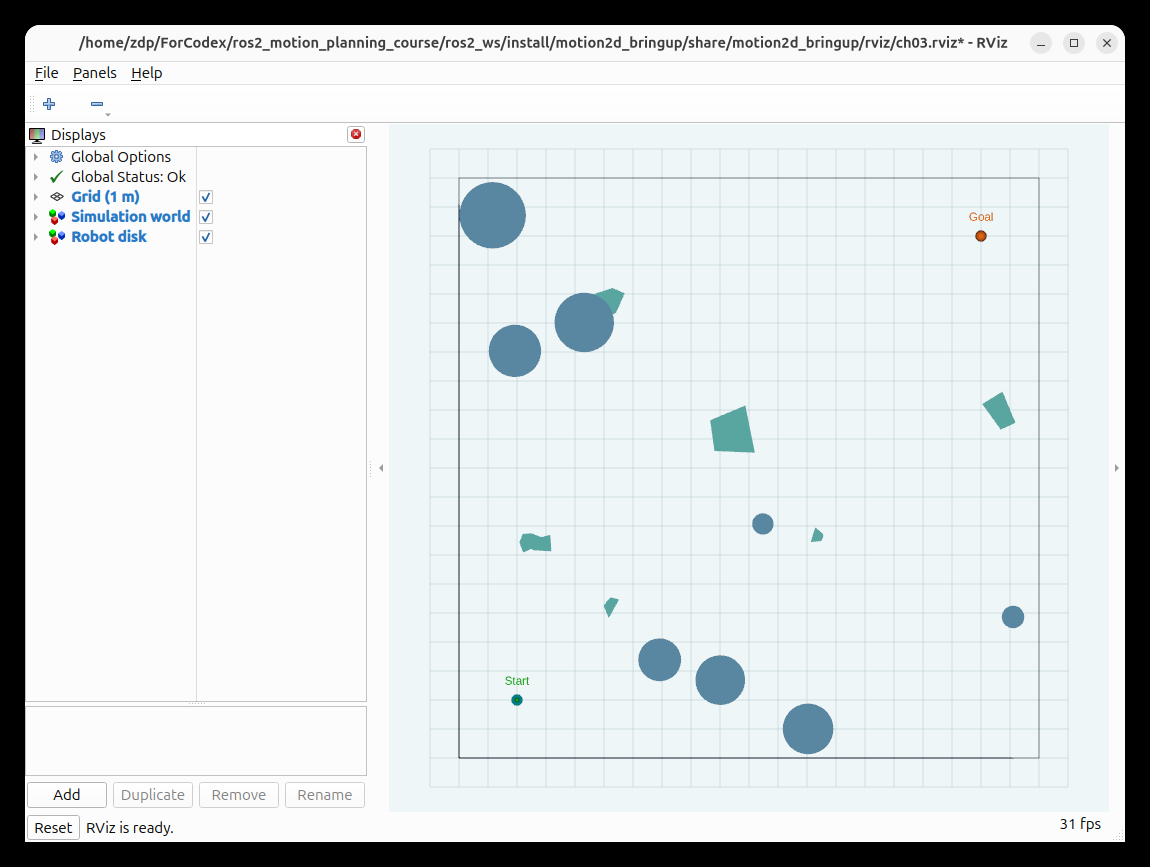
\includegraphics[width=.85\linewidth]{figures/ch03_rviz.png}
\caption{seed=42 的实际世界。圆和凸多边形可以重叠；Start 与 Goal 分别标出起终点。}
\end{figure}

\clearpage
\section{圆心不碰撞，不代表圆盘不碰撞}
半径为 r 的圆盘中心位于 p，圆形障碍中心为 c、半径为 R。两者相切时，中心距为 $r+R$，本课程把接触计为碰撞：
\begin{equation}
\|p-c\|>r+R \quad\Longleftrightarrow\quad \text{与该障碍无碰撞}.
\end{equation}
定义单个障碍的有符号距离 $d(p)$：外部为正、内部为负。自由区域中，圆盘需要 $d(p)>r$。如要额外留出安全裕量 $\delta$，使用 $d(p)>r+\delta$；物理半径与规划裕量是两个不同参数。

世界边界也限制可用空间。核心函数在自由域中取边界和所有障碍的最小距离，再比较半径：
\par\noindent\begin{minipage}{\linewidth}
\lstinputlisting[language=C++,linerange={clearance_begin-clearance_end},
  includerangemarker=false]{../ros2_ws/src/motion2d/src/sim/world.cpp}
\end{minipage}\par
占据区或越界时，这个函数用于判断符号，不承诺给出并集内部的精确 ESDF；第 12 章会专门构建距离场。

\section{点到线段的距离}
多边形边界由线段组成。设边为 $a\to b$，把点 p 投影到直线上：
\begin{equation}
t^*=\frac{(p-a)^\top(b-a)}{\|b-a\|^2},\qquad
t=\min(1,\max(0,t^*)),\qquad q=a+t(b-a).
\end{equation}
q 是线段上离 p 最近的点，距离是 $\|p-q\|$。限制 t 很重要：离线段延长线很近，不代表离有限线段很近。若 a=b，则线段退化为一个点。
\par\noindent\begin{minipage}{\linewidth}
\lstinputlisting[language=C++,linerange={distance_begin-distance_end},
  includerangemarker=false]{../ros2_ws/src/motion2d/src/geometry/obstacles.cpp}
\end{minipage}\par
对逆时针凸多边形，内部点位于每条有向边的左侧。若点在内部，距离取负；外部则取到全部边的最小距离。

\section{随机多边形为什么从凸包开始？}
随意把随机点连起来可能产生自交。我们的步骤是：在一个采样圆盘内生成点，再取凸包。可把凸包想成绕所有点拉紧的橡皮筋。实现先按 x/y 排序，再维护上、下两条只向同一方向拐弯的链。

若 $u,v$ 独立服从 $[0,1)$ 均匀分布，使用
\begin{equation}
\theta=2\pi u,\qquad \rho=R\sqrt v,\qquad
p=c+\rho(\cos\theta,\sin\theta)
\end{equation}
让采样点在圆盘面积上均匀。因为半径不超过 $\rho$ 的面积比例是 $\rho^2/R^2$，所以半径要取平方根。

代码中 \code{polygon_samples=8} 表示采样八个点，凸包顶点通常更少。校验要求顶点有限、严格凸、逆时针；对每条边检查其余顶点都位于左侧，也能排除自交星形。

不同障碍可以重叠，这仍是合法障碍并集。世界生成器只拒绝无效形状、越界和侵入起终点保护圆的候选。每个形状最多尝试 1000 次，失败明确报告，不偷偷换种子。

\section{先检查可达，再讲最短路径}
起点、终点各自无碰撞，并不意味着中间一定连通。我们先用粗网格和四邻接 flood fill 检查连通性：从起点所在格入队，反复访问相邻自由格，能到终点格即通过。它不寻找最短路径，也不替代第 11 章的 A*。

不能仅检查格中心。对于宽 $\Delta x$、高 $\Delta y$ 的单元，中心到最远角点的距离为
\begin{equation}
\epsilon_{\rm cell}=\frac12\sqrt{\Delta x^2+\Delta y^2}.
\end{equation}
中心只有在净空大于 $r+\delta+\epsilon_{\rm cell}$ 时才标为自由。这保证整个单元能容纳圆盘，代价是窄通道可能被保守拒绝。

默认检查分辨率 0.25 m。若失败，可以明确减小分辨率或关闭 \code{require_connected} 观察场景；同一个 seed 不会自动被替换成“更好看”的世界。记录失败案例也是学习的一部分。

\clearpage
\section{参数、练习与验收}
编辑 \path{ros2_ws/src/motion2d_bringup/config/ch03.yaml} 后重启。公共 x/y/radius 同时提供给坐标节点和世界节点；圆盘显示与碰撞不应使用两套不同半径。
\begin{enumerate}
\item \textbf{理解：}给一个圆心在自由空间、圆盘却碰撞的例子。解释相切和安全裕量。
\item \textbf{代码：}实现 \path{exercises/ch03/starter/segment_distance.hpp} 的点线段距离。独立检查覆盖内点、端点外、线段上和退化线段；提示与参考解单独存放。
\item \textbf{实验：}相同配置和 seed=42 启动两次，比较地图。然后改为 43，再把两类障碍各增至 20 个，记录可达性和起终点净空。
\end{enumerate}
代码练习从仓库根目录单独编译，不依赖 ROS：
\begin{lstlisting}[language=bash,numbers=none]
g++ -std=c++17 -I/usr/include/eigen3 \
  -Iexercises/ch03/starter \
  exercises/ch03/check.cpp -o /tmp/ch03_exercise
/tmp/ch03_exercise
\end{lstlisting}
将 starter 替换为 solutions 可以检验参考解。先运行未完成的练习观察失败位置，再修改投影公式；不要通过删掉检查来得到“通过”。

在同一标准库和参数下，固定种子复现相同世界；跨编译器标准库版本不保证分布函数的逐位一致。输出状态说明是否执行了连通性检查，避免把“没有检查”当成“已经通过”。

运行 \code{colcon test} 检查几何、碰撞和可达性；演示运行时，在工作空间执行以下命令核对默认消息：
\begin{lstlisting}[language=bash,numbers=none]
/usr/bin/python3 ../scripts/check_ch03.py
\end{lstlisting}
RViz2 展示全部障碍、边界和起终点，图形并非激光建图结果。

\begin{notebox}
\textbf{常见问题}

看不见障碍时，先确认 Fixed Frame 为 map、World 的话题为
\code{/visualization/world}，再检查节点有没有因无效参数退出。改参数后要重启；
本章尚不提供运行中重建世界。若可达性检查失败，保留 seed 和配置，再研究分辨率与通道宽度。
\end{notebox}
